\documentclass[12pt, a4paper]{article}
\usepackage{ctex} % 中文的宏包
\usepackage{indentfirst}
\usepackage{graphicx} % 插入圖片的宏包
\usepackage{float} % 設置圖片浮動位置的宏包
\usepackage{subfigure} % 插入多圖時用子圖顯示宏包
\usepackage{listings} % 代碼塊宏包
\usepackage{color} % 代碼高亮
\usepackage[colorlinks,linkcolor=blue]{hyperref} % URL 包

\definecolor{dkgreen}{rgb}{0,0.6,0}
\definecolor{gray}{rgb}{0.5,0.5,0.5}
\definecolor{mauve}{rgb}{0.58,0,0.82}

\lstset{ %
    %language=Octave,                % the language of the code
    basicstyle=\scriptsize\Hack,           % the size of the fonts that are used for the code
    numbers=none,                   % where to put the line-numbers
    numberstyle=\tiny\color{gray},  % the style that is used for the line-numbers
    stepnumber=2,                   % the step between two line-numbers. If it's 1, each line 
                                    % will be numbered
    numbersep=3pt,                  % how far the line-numbers are from the code
    backgroundcolor=\color{white},      % choose the background color. You must add \usepackage{color}
    showspaces=false,               % show spaces adding particular underscores
    showstringspaces=false,         % underline spaces within strings
    showtabs=false,                 % show tabs within strings adding particular underscores
    frame=single,                   % adds a frame around the code
    rulecolor=\color{black},        % if not set, the frame-color may be changed on line-breaks within not-black text (e.g. commens (green here))
    tabsize=2,                      % sets default tabsize to 2 spaces
    captionpos=b,                   % sets the caption-position to bottom
    breaklines=true,                % sets automatic line breaking
    breakatwhitespace=false,        % sets if automatic breaks should only happen at whitespace
    title=\lstname,                   % show the filename of files included with \lstinputlisting;
                                    % also try caption instead of title
    keywordstyle=\color{blue},          % keyword style
    commentstyle=\color{dkgreen},       % comment style
    stringstyle=\color{mauve},         % string literal style
    escapeinside={\%*}{*},            % if you want to add LaTeX within your code
    morekeywords={*,...}               % if you want to add more keywords to the set
}
\setCJKmainfont{Noto Serif CJK TC} % 主要字體 Noto Serif
\newfontfamily\Hack{Hack} % 代碼字體
\author{Huang Po Hsun}
\date{\today}
\title{在 Linux 上控制 Python 版本 - Pyenv}
\begin{document}
\maketitle
\begin{figure}[H] % H 為當前位置,!htb 為忽略美學標準,htbp 為浮動圖片
    \centering % 圖片居中
    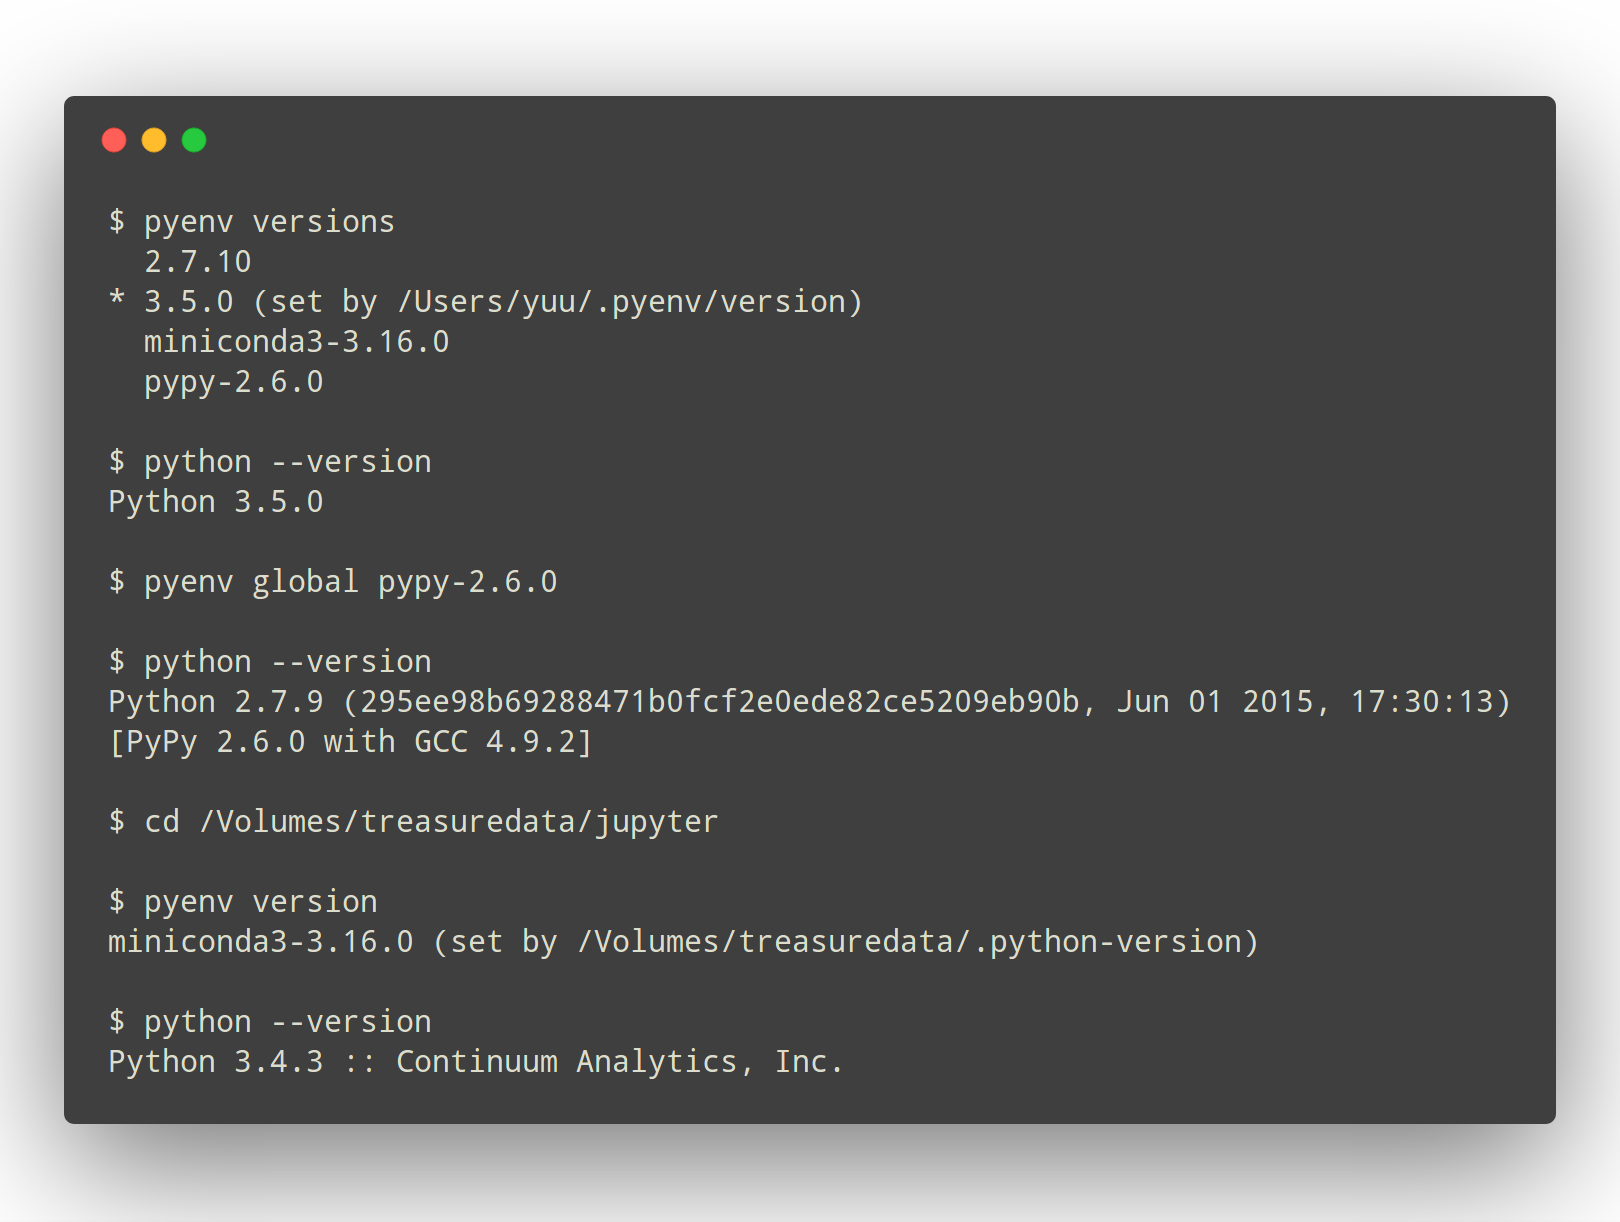
\includegraphics[width=1\textwidth]{terminal_output.png} % 插入圖片,[] 為圖片大小,{} 是圖片文件
\end{figure}
\newpage
\section{前言}
    在 Linux 開發 Python 相關的項目,你是不是會碰到關於 Python 版本之類的問題?像是開發 Tensorflow 的時候碰到版本問題,{\bf 原本 Python 3.7 可以支援 Tensorflow,
    但是忽然 Python 從 3.7 更新到 3.8.0},這時 Python 3.8 不支援 Tensorflow,你苦惱了,千辛萬苦的項目因為系統更新而導致版本不支援使項目暫停開發,
    這時 pyenv 將成為你的救星,如果你硬是不肯更新系統 Python 版本,你的系統將會得不到最新的體驗與安全並處於危險的不穩定狀態,系統更新真的很重要。

    {\bf pyenv 是很棒的 Python 版本控制工具,讓你的電腦可以安裝多個 Python 版本。}\href{https://github.com/pyenv/pyenv}{pyenv} 是 Github 上的開源項目,
    關於使用須知該項目的 README.md 寫得很詳細。我這篇文章就分享一下我在 Arch Linux 的安裝方式。
\section{安裝}

    從 Github 倉庫上直接 clone 下來。你也可以選擇直接在瀏覽器上下來。然後壓縮包解壓將文件內的文件放入 {\Hack{$\sim/.pyenv$}}。

    \subsection{設置代理}
        {\footnotesize 註:如果你在國內網使用 Github 網速過於緩慢,建議開 Proxy,然後給 \href{https://gist.github.com/laispace/666dd7b27e9116faece6}{Git 設置代理}。}

        \begin{lstlisting}[title=Git 設置代理, frame=shadowbox, language=Octave]
            # set http
            git config --global http.proxy 'socks5://127.0.0.1:1080'
            # set https
            git config --global https.proxy 'socks5://127.0.0.1:1080'
            # unset http
            git config --global --unset http.proxy
            # unset https
            git config --global --unset https.proxy

            npm config delete proxy
        \end{lstlisting}
    \subsection{下載}
        \begin{lstlisting}[basicstyle=\tiny\Hack, language=Octave]
            git clone https://github.com/pyenv/pyenv.git ~/.pyenv # Basic GitHub Checkout
        \end{lstlisting}
\section{環境變量}
    \subsection{PYENV\underline{ }ROOT}
        將 PYENV\underline{ }ROOT 添加至環境變量。在 Konsole 輸入以下指令:

        {\footnotesize 註:在 Arch 發行版中,$\sim/.bash\underline{ }profile$ 就是 $\sim/.profile$。如果你 Shell 使用的是 {\bf ZSH},
        為了在 {\bf ZSH} 中也能使用,記得也要寫入 $\sim/.zshrc$。之所以要求要兩個都寫入是因為避免如果你如果換了其它 Shell 需要再重新設一次。}\\[0.5mm]

        \begin{lstlisting}[language=Octave]
            # .profile
            echo 'export PYENV_ROOT="$HOME/.pyenv"' >> ~/.profile
            echo 'export PATH="$PYENV_ROOT/bin:$PATH"' >> ~/.profile
            # .zshrc
            echo 'export PYENV_ROOT="$HOME/.pyenv"' >> ~/.zshrc
            echo 'export PATH="$PYENV_ROOT/bin:$PATH"' >> ~/.zshrc
        \end{lstlisting}
    \subsection{pyenv init}
        將 pyenv init 添加到您的 Shell 中以啟用填充和自動補全功能。 
        請確保將 \texttt{\Hack{eval "\$(pyenv init-)"}} 放在 Shell 配置文件的末尾,
        因為它在初始化期間會操縱 PATH 。\\[0.01mm]

        \begin{lstlisting}[basicstyle=\tiny\Hack, language=Octave]
            # .profile
            echo -e 'if command -v pyenv 1>/dev/null 2>&1; then\n  eval "$(pyenv init -)"\nfi' >> ~/.profile
            # .zshrc
            echo -e 'if command -v pyenv 1>/dev/null 2>&1; then\n  eval "$(pyenv init -)"\nfi' >> ~/.zshrc
        \end{lstlisting}
\section{重啟 SHELL}
    先重新加載環境變量文件後,重啟 Shell。\\[0.01mm]

    \begin{lstlisting}[language=Octave]
        source ~/.profile
        source ~/.zshrc
    \end{lstlisting}

    接下來你輸入 \texttt{pyenv version},應該就會顯示你目前 pyenv 使用的 Python 版本,
    輸入 \texttt{pyenv versions} 能顯示你 pyenv 中安裝的所有 Python 版本。
\section{安裝 Python 版本}
    我目前要使用 Python 3.7.6 的版本。\\[0.01mm]
    \begin{lstlisting}[language=Octave]
        pyenv install 3.7.6
    \end{lstlisting}
\section{設置 Shell 默認全局 Python 版本}
    \begin{lstlisting}[language=Octave]
        pyenv global 3.7.6
    \end{lstlisting}
    接下來重新登出登入電腦。使用 \texttt{python --version} 查看 Python 版本就會發現版本已經變成 3.7.6 了。
\section{Reference}
    \begin{itemize}
        \item \href{https://github.com/pyenv/pyenv}{pyenv / pyenv - Github}
        \item \href{https://gist.github.com/laispace/666dd7b27e9116faece6}{Git 設置與取消代理}
    \end{itemize}
\end{document}